
\section{Apache CloudStack}

Apache CloudStack is an open source that provides a highly scalable
and available cloud management platform for IT Enterprises and service
providers. CloudStack was originally developed by Cloud.com and was
known by the name VMOps.  In 2011, Citrix acquired the product and
donated it to Apache.  ``CloudStack is being developed to help managed
service providers and enterprise IT departments create and operate
public cloud, private cloud or hybrid clouds with capabilities
equivalent to Amazon's Elastic Compute Cloud (Amazon EC2) It uses
existing hypervisors such as KVM, VMware ESXi|VMware vcenter and
XenServer/XCP for virtualization. In addition to its own API,
CloudStack also supports the Amazon Web Services (AWS) API[3] and the
Open Cloud Computing Interface from the Open Grid
Forum.''~\cite{hid-sp18-417-wiki-cloudStack}.  The key feature of the
product are (1) high availability of resources (2) network management
(3) provides GUI for ease of management (4) compatible with most of
the hypervisor/virtual monitor (5) it provides the snapshot
management. e.g.\ This feature is very useful is saving a state
[snapshot] of a vitual machine.  The vm can later be reverted to the
stored state.  The basic deployment of CloudStack just needs two
machines: A server and a hypervisor that is a monitoring system.  The
process can be over simplified by configuring one machine to serve
both the purpose.  The same simple system can easily be scaled to a
zone or a pod.  Figure~\ref{F:cloudstack-scalabuility} depicts how the
simplest deployment infrastructure can be scaled to provide an
advanced support system.


\begin{figure}[htb]
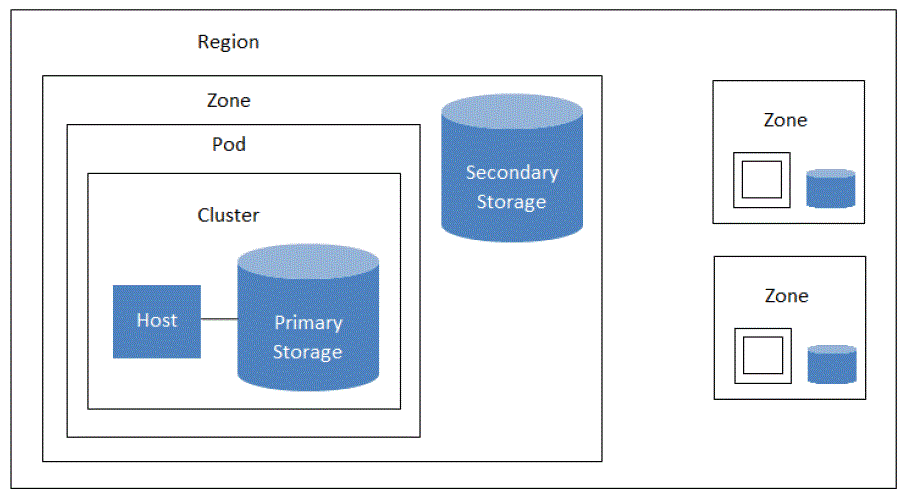
\includegraphics[width=\textwidth]{images/hid-sp18-417-cloudstack.png}
\caption{CloudStack Scalability~\cite{hid-sp18-417-cloudstack-scaling}}
\label{F:cloudstack-scalabuility}
\end{figure}
